\subsection{Product Quality Requirements}

This section defines the non-functional characteristics of CookWise through five quality requirements covering accuracy, reliability, performance, usability, and scalability. Each requirement is specified as a measurable "shall" statement with defined validation procedures.

\subsubsection{Quality Requirements Summary}

Table \ref{tab:qr_summary} presents all quality requirements for the CookWise system:

\begin{table}[H]
\centering
\caption{CookWise Quality Requirements Summary}
\label{tab:qr_summary}
\begin{tabular}{|p{1.5cm}|p{3cm}|p{8.5cm}|p{1.5cm}|}
\hline
\textbf{ID} & \textbf{Quality Aspect} & \textbf{Requirement} & \textbf{Target} \\
\hline
QR1 & Accuracy & The system shall achieve at least 95\% accuracy in sale price data, measured as the percentage of sale prices that match actual retailer prices. & 95\% \\
\hline
QR2 & Reliability & The system shall maintain at least 98\% uptime during peak usage hours (17:00-20:00 local time), measured as the percentage of time the application is fully operational and accessible. & 98\% \\
\hline
QR3 & Performance & The system shall generate recipe suggestions within 5 seconds for 95\% of user requests, measured from the time a user submits search criteria to when results are displayed. & 5 sec \\
\hline
QR4 & Usability & The system shall enable new users to complete their first recipe selection within 8 minutes of account creation, measured from login to adding a recipe to their shopping list. & 8 min \\
\hline
QR5 & Scalability & The system shall support at least 300 concurrent users while maintaining acceptable performance (response time under 10 seconds), measured during peak usage hours. & 300 users \\
\hline
\end{tabular}
\end{table}

\vspace{0.3cm}

\textbf{QUPER Analysis Approach:} Two quality requirements (QR1 and QR5) undergo detailed QUPER analysis due to their complexity and cost implications, while QR2, QR3, and QR4 have straightforward targets.

\subsubsection{QR1: Accuracy - Price Data Correctness (QUPER Analysis)}

\textbf{Requirement:} The system shall achieve at least 95\% accuracy in sale price data, measured as the percentage of ingredient sale prices that match actual current sale prices published by retailers.

\vspace{0.2cm}

\textbf{Rationale:} Accuracy is critical for user trust and cost savings. Different accuracy levels require different technical approaches, making QUPER analysis valuable for understanding cost benefit tradeoffs.

\begin{table}[H]
\centering
\begin{tabular}{|p{14cm}|}
\hline
\textbf{FEATURE:} Sale Price Information \\
\textbf{ID:} QR1 \\
\textbf{QUALITY REQUIREMENT:} Accuracy of sale prices \\
\hline
\textbf{DEFINITION:} The percentage of ingredient sale prices in the application that match the actual current sale prices published by retailers, measured as (number of correct prices / total number of sale prices) × 100. \\
\hline
\textbf{REFERENCE LEVELS} \\
\textbf{PRODUCT:} eTilbudsavis \textbf{LEVEL:} 95\% accuracy \\
\textbf{PRODUCT:} Price comparison websites \textbf{LEVEL:} 85-90\% accuracy \\
\textbf{PRODUCT:} Current CookWise \textbf{LEVEL:} N/A (new system) \\
\hline
\textbf{QUALITY BREAKPOINTS} \\
\textbf{UTILITY:} 90\% accuracy \textbf{RATIONALE:} Below 90\%, users lose trust in recommendations. One in ten incorrect prices creates too many negative experiences and undermines cost savings value proposition. \\
\textbf{SATURATION:} 100\% accuracy \textbf{RATIONALE:} Perfect accuracy impossible with web scraping due to timing delays, retailer website changes, and regional variations. Diminishing returns beyond 98-99\%. \\
\textbf{DIFFERENTIATION:} 98\% accuracy \textbf{RATIONALE:} Accuracy of 98\%+ establishes application as highly reliable and trustworthy. Can be promoted as "verified sale prices" for strong competitive advantage. \\
\hline
\textbf{COST BARRIERS AND TECHNIQUES} \\
\textbf{Qref:} 92\% accuracy - Basic web scraping with simple validation \\
\textbf{Q1:} 96\% accuracy \textbf{RATIONALE:} Advanced parsing algorithms, automated validation checks, error detection and correction systems. Requires sophisticated data validation logic for multiple retailer formats. Moving beyond 96\% requires switching to or supplementing with API integrations instead of web scraping alone. \\
\textbf{C1:} 2 weeks \\
\textbf{Q2:} 99\% accuracy \textbf{RATIONALE:} Multi-source validation combining web scraping with retailer API access (where available), cross-verification against multiple data points, and machine learning for anomaly detection. Requires partnerships with retailers and sophisticated data reconciliation. \\
\textbf{C2:} 16 weeks \\
\hline
\textbf{TARGETS} \\
\textbf{GOOD:} 95\% accuracy \textbf{RATIONALE:} Reliable enough for confident purchasing decisions, matches best available competitor (eTilbudsavis), achievable with robust web scraping implementation and validation checks. \\
\textbf{STRETCH:} 97\% accuracy \textbf{RATIONALE:} Provides differentiation through advanced web scraping techniques, automated error correction, and multi-source data validation systems. \\
\hline
\textbf{VALIDATION PROCEDURE} \\
Accuracy validated through weekly manual verification tests. Random sample of 100 sale items selected from database and manually checked against current retailer websites and physical store flyers. Percentage of matching prices calculated. Additionally, users can report incorrect prices through application for ongoing accuracy monitoring. \\
\hline
\end{tabular}
\caption{QR1: Accuracy Quality Requirement with QUPER Analysis}
\label{tab:qr1}
\end{table}

\begin{figure}[H]
    \centering
    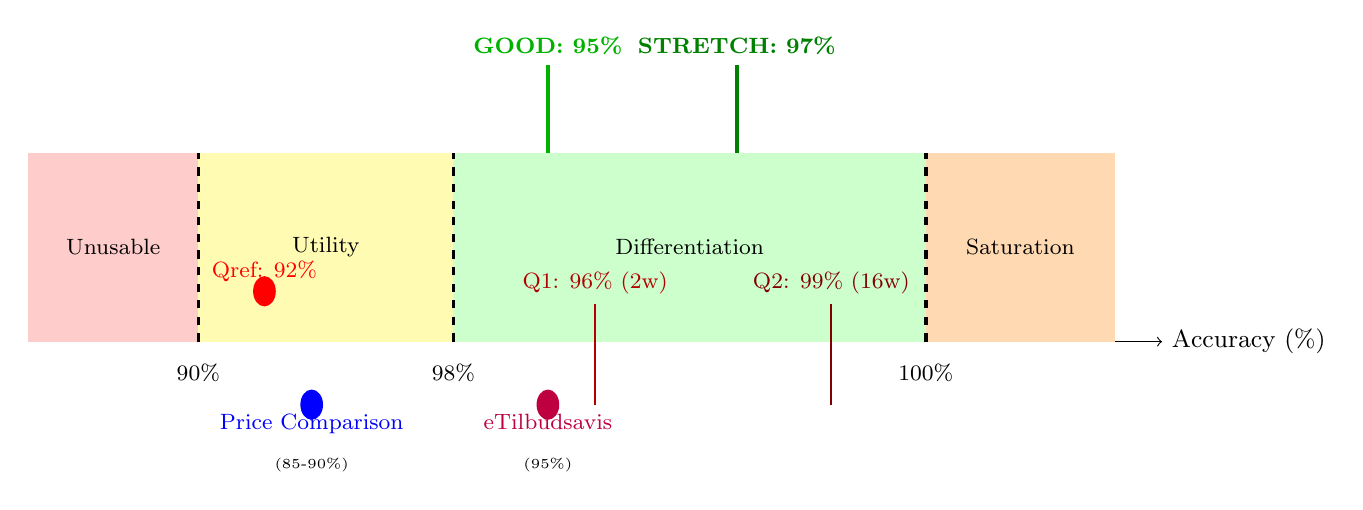
\begin{tikzpicture}[xscale=1.2, yscale=1.6]
        % Quality axis
        \draw[->] (0,0) -- (12,0) node[right] {\small Accuracy (\%)};

        % Three zones with colors
        \fill[red!20] (0,0) rectangle (1.8,1.5);
        \fill[yellow!30] (1.8,0) rectangle (4.5,1.5);
        \fill[green!20] (4.5,0) rectangle (9.5,1.5);
        \fill[orange!30] (9.5,0) rectangle (11.5,1.5);

        % Zone labels
        \node[font=\footnotesize] at (0.9,0.75) {Unusable};
        \node[font=\footnotesize] at (3.15,0.75) {Utility};
        \node[font=\footnotesize] at (7,0.75) {Differentiation};
        \node[font=\footnotesize] at (10.5,0.75) {Saturation};

        % Breakpoint lines
        \draw[very thick, dashed] (1.8,0) -- (1.8,1.5);
        \draw[very thick, dashed] (4.5,0) -- (4.5,1.5);
        \draw[very thick, dashed] (9.5,0) -- (9.5,1.5);

        % Axis labels for breakpoints
        \node[below, font=\footnotesize] at (1.8,-0.1) {90\%};
        \node[below, font=\footnotesize] at (4.5,-0.1) {98\%};
        \node[below, font=\footnotesize] at (9.5,-0.1) {100\%};

        % Competitor and product markers
        \fill[blue] (3,-0.5) circle (0.12) node[below, font=\footnotesize] {Price Comparison};
        \node[below, font=\tiny] at (3,-0.85) {(85-90\%)};
        \fill[purple] (5.5,-0.5) circle (0.12) node[below, font=\footnotesize] {eTilbudsavis};
        \node[below, font=\tiny] at (5.5,-0.85) {(95\%)};
        \fill[red] (2.5,0.4) circle (0.12) node[above, font=\footnotesize] {Qref: 92\%};

        % Cost barriers
        \draw[thick, red!70!black] (6,-0.5) -- (6,0.3);
        \node[above, font=\footnotesize, red!70!black] at (6,0.3) {Q1: 96\% (2w)};

        \draw[thick, red!50!black] (8.5,-0.5) -- (8.5,0.3);
        \node[above, font=\footnotesize, red!50!black] at (8.5,0.3) {Q2: 99\% (16w)};

        % Targets
        \draw[very thick, green!70!black] (5.5,1.5) -- (5.5,2.2);
        \node[above, font=\footnotesize\bfseries, green!70!black] at (5.5,2.2) {GOOD: 95\%};

        \draw[very thick, green!50!black] (7.5,1.5) -- (7.5,2.2);
        \node[above, font=\footnotesize\bfseries, green!50!black] at (7.5,2.2) {STRETCH: 97\%};

    \end{tikzpicture}
    \caption{QUPER Roadmap for QR1: Accuracy (Price Data Correctness)}
    \label{fig:qr1_roadmap}
\end{figure}

\textbf{Saturation Interpretation:} Beyond 98\%, each additional percentage point requires exponentially increasing effort with minimal user perceived benefit.

\subsubsection{QR5: Scalability - Concurrent User Capacity (QUPER Analysis)}

\textbf{Requirement:} The system shall support at least 300 concurrent users while maintaining acceptable performance (response time under 10 seconds), measured during peak usage hours.

\vspace{0.2cm}

\textbf{Rationale:} Scalability requires QUPER analysis because infrastructure costs increase significantly at different capacity levels, and target selection involves substantial infrastructure investment decisions.

\begin{table}[H]
\centering
\begin{tabular}{|p{14cm}|}
\hline
\textbf{FEATURE:} System Infrastructure \\
\textbf{ID:} QR5 \\
\textbf{QUALITY REQUIREMENT:} Concurrent user support \\
\hline
\textbf{DEFINITION:} The maximum number of users who can simultaneously use the application while maintaining acceptable performance (response time under 10 seconds), measured during peak usage hours. \\
\hline
\textbf{REFERENCE LEVELS} \\
\textbf{PRODUCT:} Small recipe apps \textbf{LEVEL:} 100-500 concurrent users \\
\textbf{PRODUCT:} eTilbudsavis scale \textbf{LEVEL:} 1000+ concurrent users \\
\textbf{PRODUCT:} Current CookWise \textbf{LEVEL:} N/A (new system) \\
\hline
\textbf{QUALITY BREAKPOINTS} \\
\textbf{UTILITY:} 50 concurrent users \textbf{RATIONALE:} Minimum viable capacity for initial launch in Swedish market. Below this, system cannot support even limited regional adoption and MVP launch becomes impractical. \\
\textbf{SATURATION:} 5000 concurrent users \textbf{RATIONALE:} Capacity beyond 5000 exceeds realistic projections for initial Swedish market penetration. Infrastructure investment at this scale cannot be justified for early-stage product. \\
\textbf{DIFFERENTIATION:} 500 concurrent users \textbf{RATIONALE:} Capacity of 500 supports significant market share in target regions (Karlskrona and surrounding areas) and enables positive growth trajectory. \\
\hline
\textbf{COST BARRIERS AND INFRASTRUCTURE INVESTMENT} \\
\textbf{Qref:} 100 concurrent users - Basic single-server deployment \\
\textbf{Q1:} 500 concurrent users \textbf{RATIONALE:} Load balancing, database connection pooling, query optimization, caching layer. Requires significant architecture improvements and database tuning. \textbf{Infrastructure cost implications:} Upgrading from shared hosting to dedicated server or basic cloud infrastructure (estimated additional \euro{}200-400/month operational costs). \\
\textbf{C1:} 3 weeks \\
\textbf{Q2:} 2000 concurrent users \textbf{RATIONALE:} Cloud infrastructure (AWS/Azure), CDN integration, distributed caching, auto-scaling. Requires migration to enterprise cloud platform and distributed system architecture. \textbf{Infrastructure cost implications:} Enterprise cloud tier with auto-scaling, load balancers, CDN (estimated additional \euro{}800-1500/month operational costs). \\
\textbf{C2:} 10 weeks \\
\hline
\textbf{TARGETS} \\
\textbf{GOOD:} 300 concurrent users \textbf{RATIONALE:} Realistic capacity for successful initial market launch, provides buffer for unexpected usage spikes, achievable with solid implementation and moderate infrastructure investment. \\
\textbf{STRETCH:} 500 concurrent users \textbf{RATIONALE:} Provides differentiation and growth capacity. Reaching this level requires infrastructure investment (approximately \euro{}200-400/month additional operational costs) which must be evaluated against project budget and expected user growth trajectory. \\
\hline
\textbf{VALIDATION PROCEDURE} \\
Scalability tested using load testing tools (Apache JMeter or Locust) simulating multiple concurrent users performing typical tasks (searching recipes, creating shopping lists). Tests gradually increase concurrent users until response time exceeds 10 seconds or error rate exceeds 1\%. Maximum concurrent users before performance degradation recorded. Testing conducted in staging environment mirroring production configuration. \\
\hline
\end{tabular}
\caption{QR5: Scalability Quality Requirement with QUPER Analysis}
\label{tab:qr5}
\end{table}

\textbf{Note on Infrastructure Costs:} Scaling from the Good level (300 users) to the Stretch level (500 users) involves both one time development costs and recurring monthly infrastructure expenses.

\subsubsection{QR2, QR3, QR4: Additional Quality Requirements}

The following quality requirements have straightforward targets based on industry standards and user expectations, and do not require detailed QUPER analysis:

\vspace{0.3cm}

\textbf{QR2: Reliability - System Uptime}
\begin{itemize}
    \item \textbf{Requirement:} The system shall maintain at least 98\% uptime during peak usage hours (17:00-20:00 local time).
    \item \textbf{Validation:} Uptime monitored using automated health checks every 60 seconds. Downtime incidents logged and analyzed. Monthly uptime percentage calculated as (total available minutes / total minutes in peak hours) × 100.
    \item \textbf{Rationale:} 98\% uptime is acceptable for MVP launch while maintaining user trust.
\end{itemize}

\vspace{0.3cm}

\textbf{QR3: Performance - Recipe Generation Response Time}
\begin{itemize}
    \item \textbf{Requirement:} The system shall generate recipe suggestions within 5 seconds for 95\% of user requests.
    \item \textbf{Validation:} Response times logged for all recipe suggestion requests. 95th percentile response time calculated weekly from logs. Measured from user search submission to complete result display.
    \item \textbf{Rationale:} Users expect web applications to respond within 5 seconds for satisfactory engagement.
\end{itemize}

\vspace{0.3cm}

\textbf{QR4: Usability - Time to First Recipe Selection}
\begin{itemize}
    \item \textbf{Requirement:} The system shall enable new users to complete their first recipe selection within 8 minutes of account creation.
    \item \textbf{Validation:} User session analytics track time from login to first recipe added to shopping list. Median completion time calculated monthly from new user cohorts. Users unable to complete task within 15 minutes flagged for usability investigation.
    \item \textbf{Rationale:} 8 minutes is a reasonable timeframe for new users to explore the interface and make their first selection.
\end{itemize}
